\begin{figure}[H]\centering
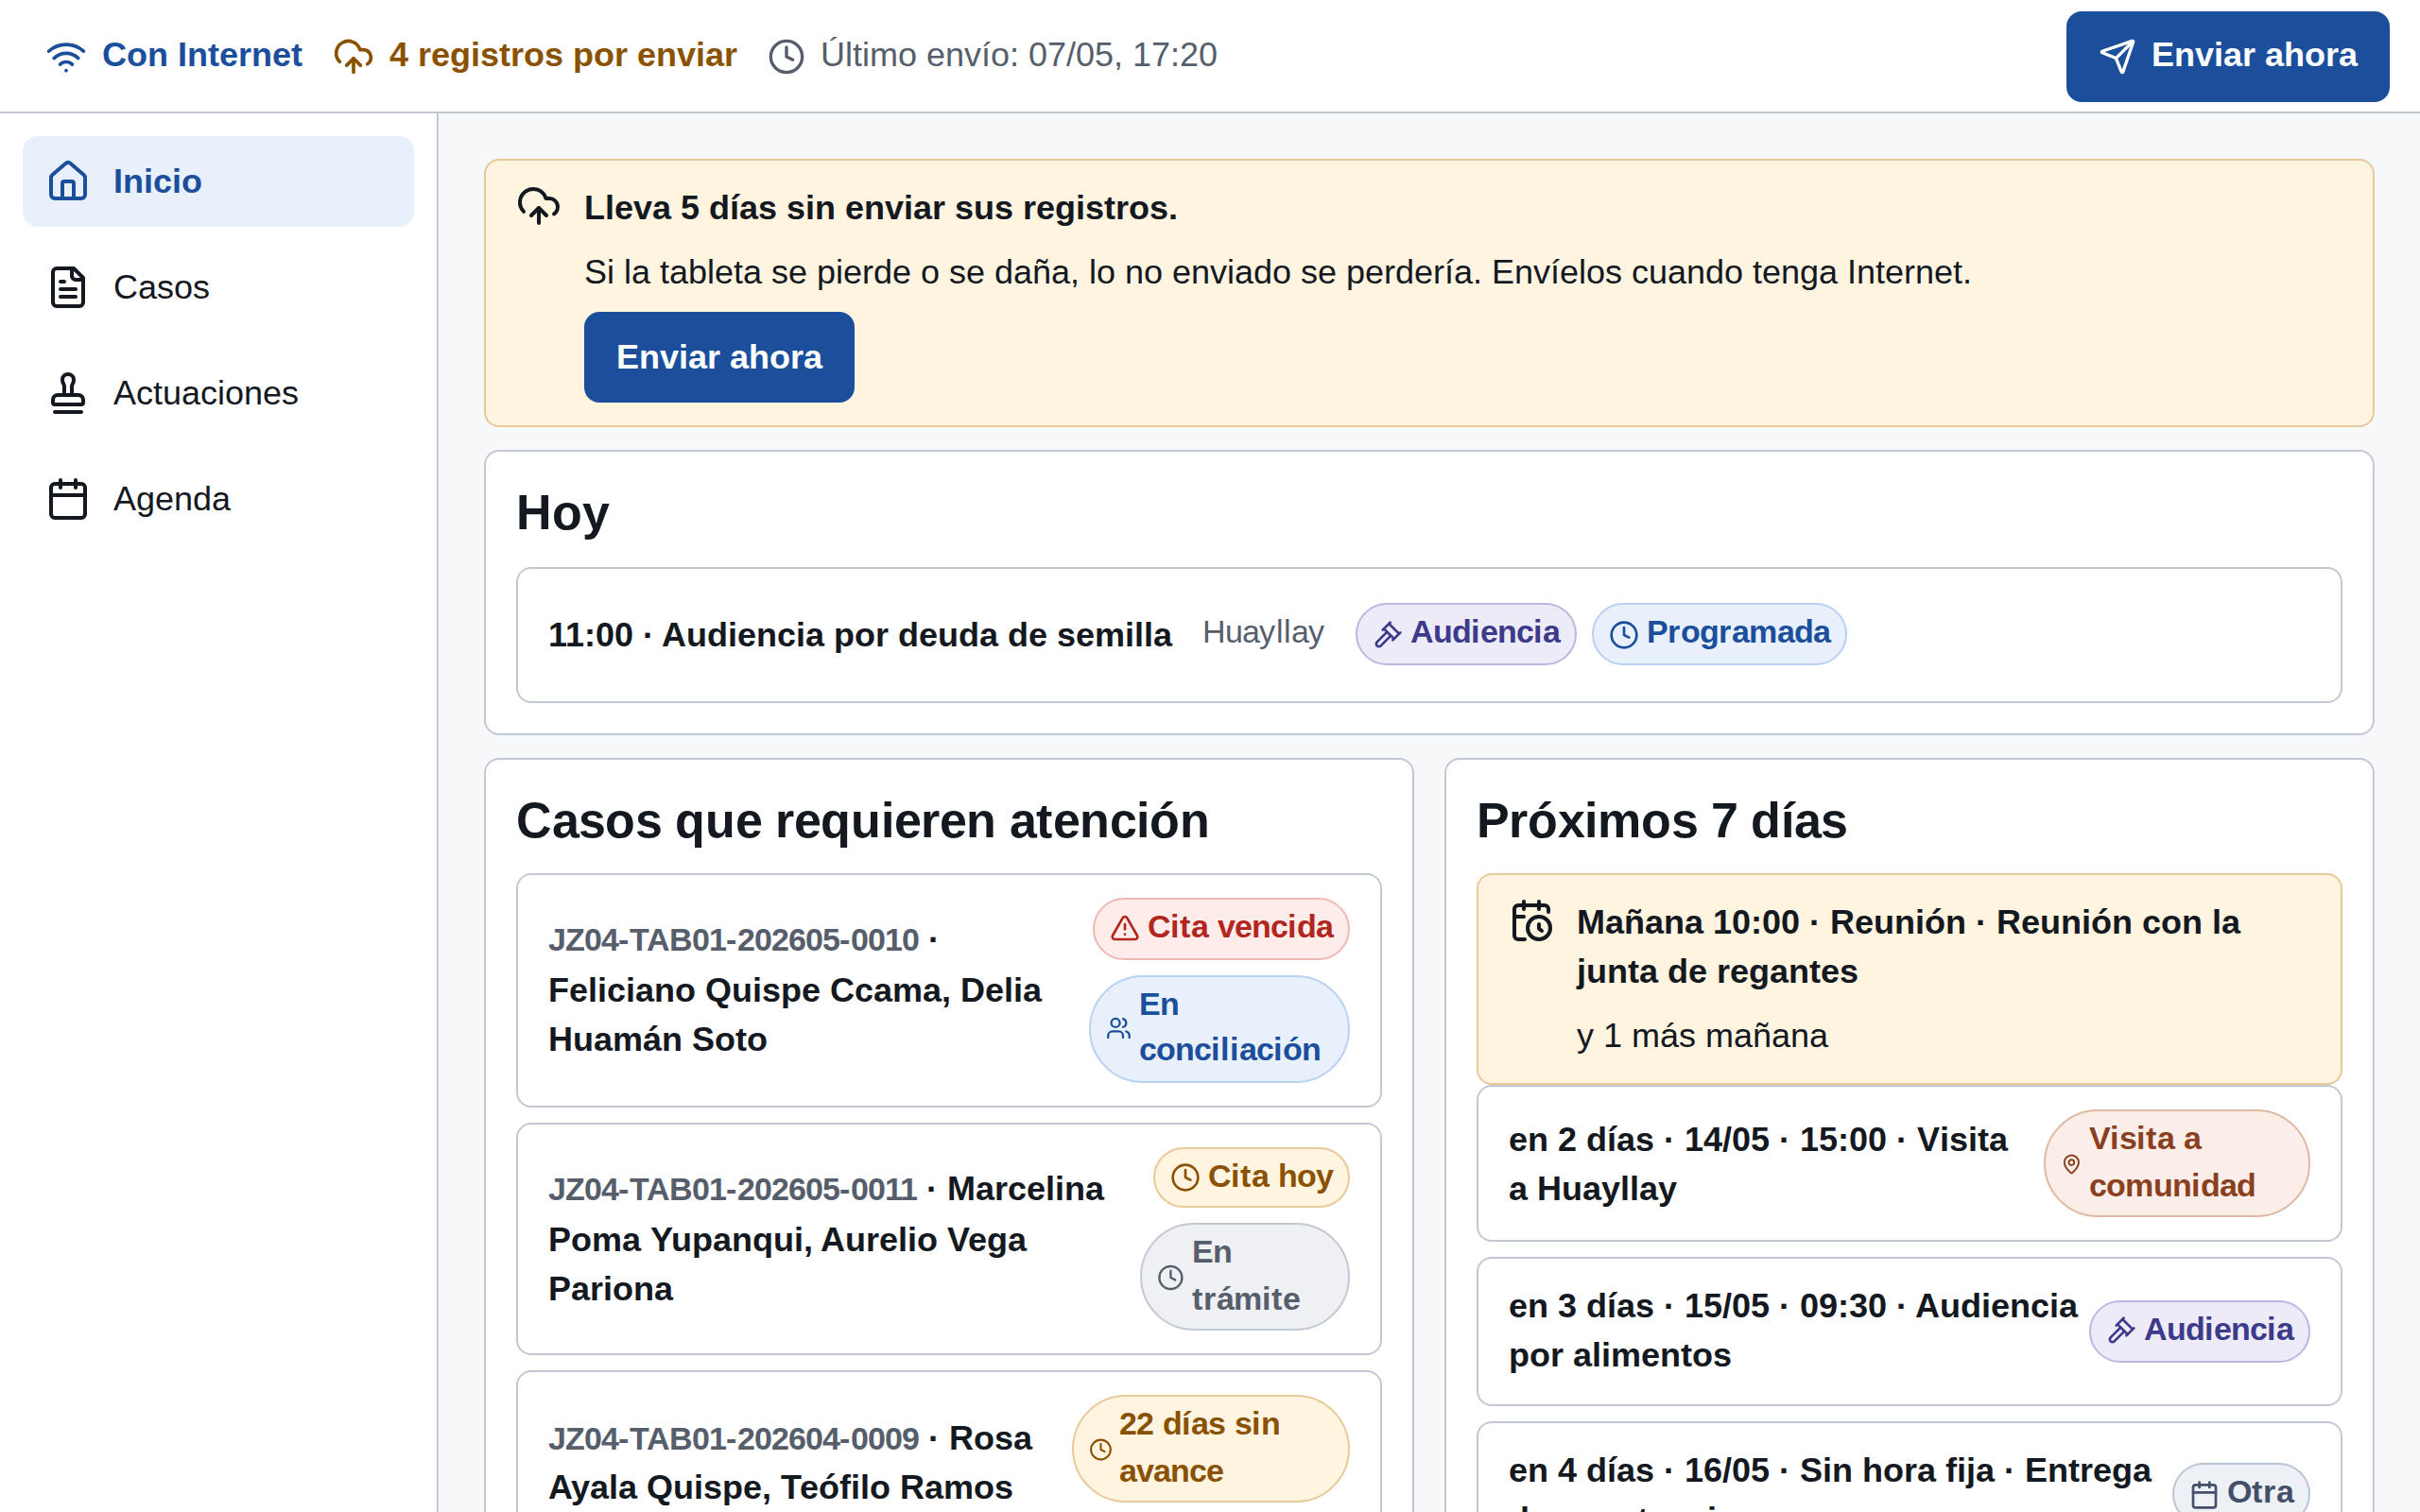
\includegraphics[width=0.78\linewidth]{capturas/X-01_recordatorio-dias.png}
\caption{P-01 · Días sin enviar. Recordatorio con el riesgo explicado en una frase, no una alarma}
\end{figure}
\begin{figure}[H]\centering
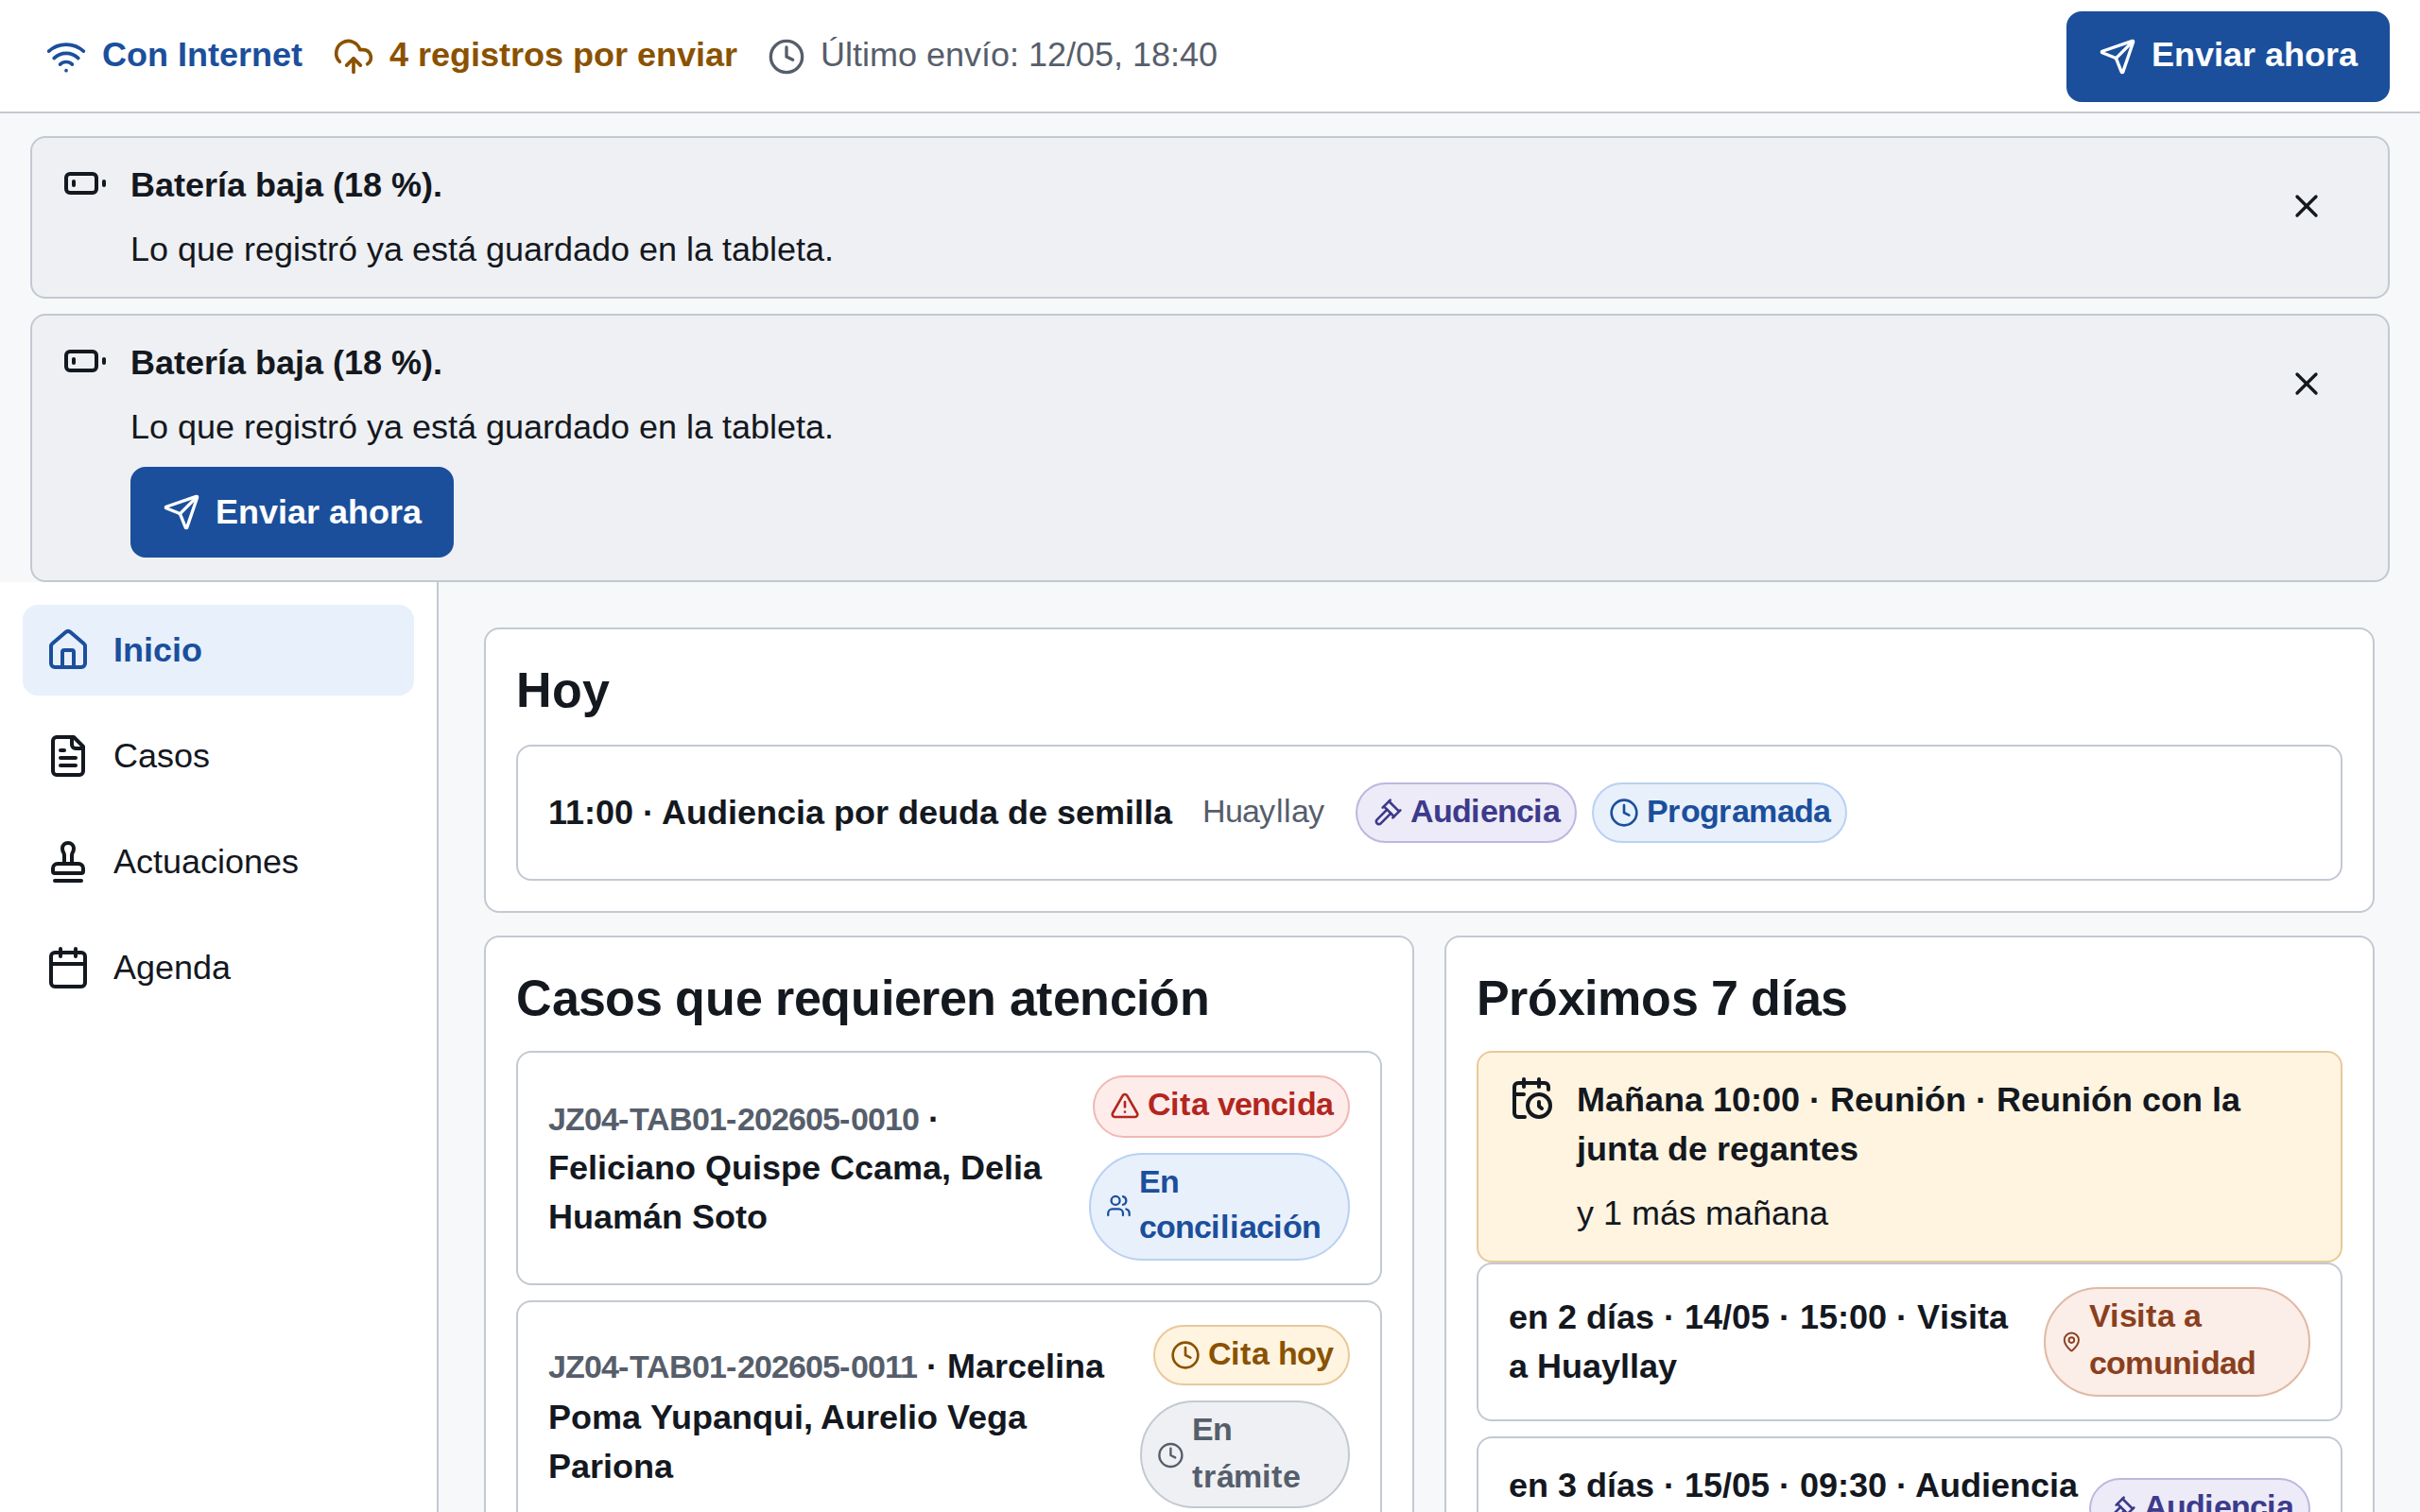
\includegraphics[width=0.78\linewidth]{capturas/X-02_bateria-20.png}
\caption{P-01 · Batería al 20 \%. Aviso de batería que recuerda que lo registrado ya está guardado}
\end{figure}
\begin{figure}[H]\centering
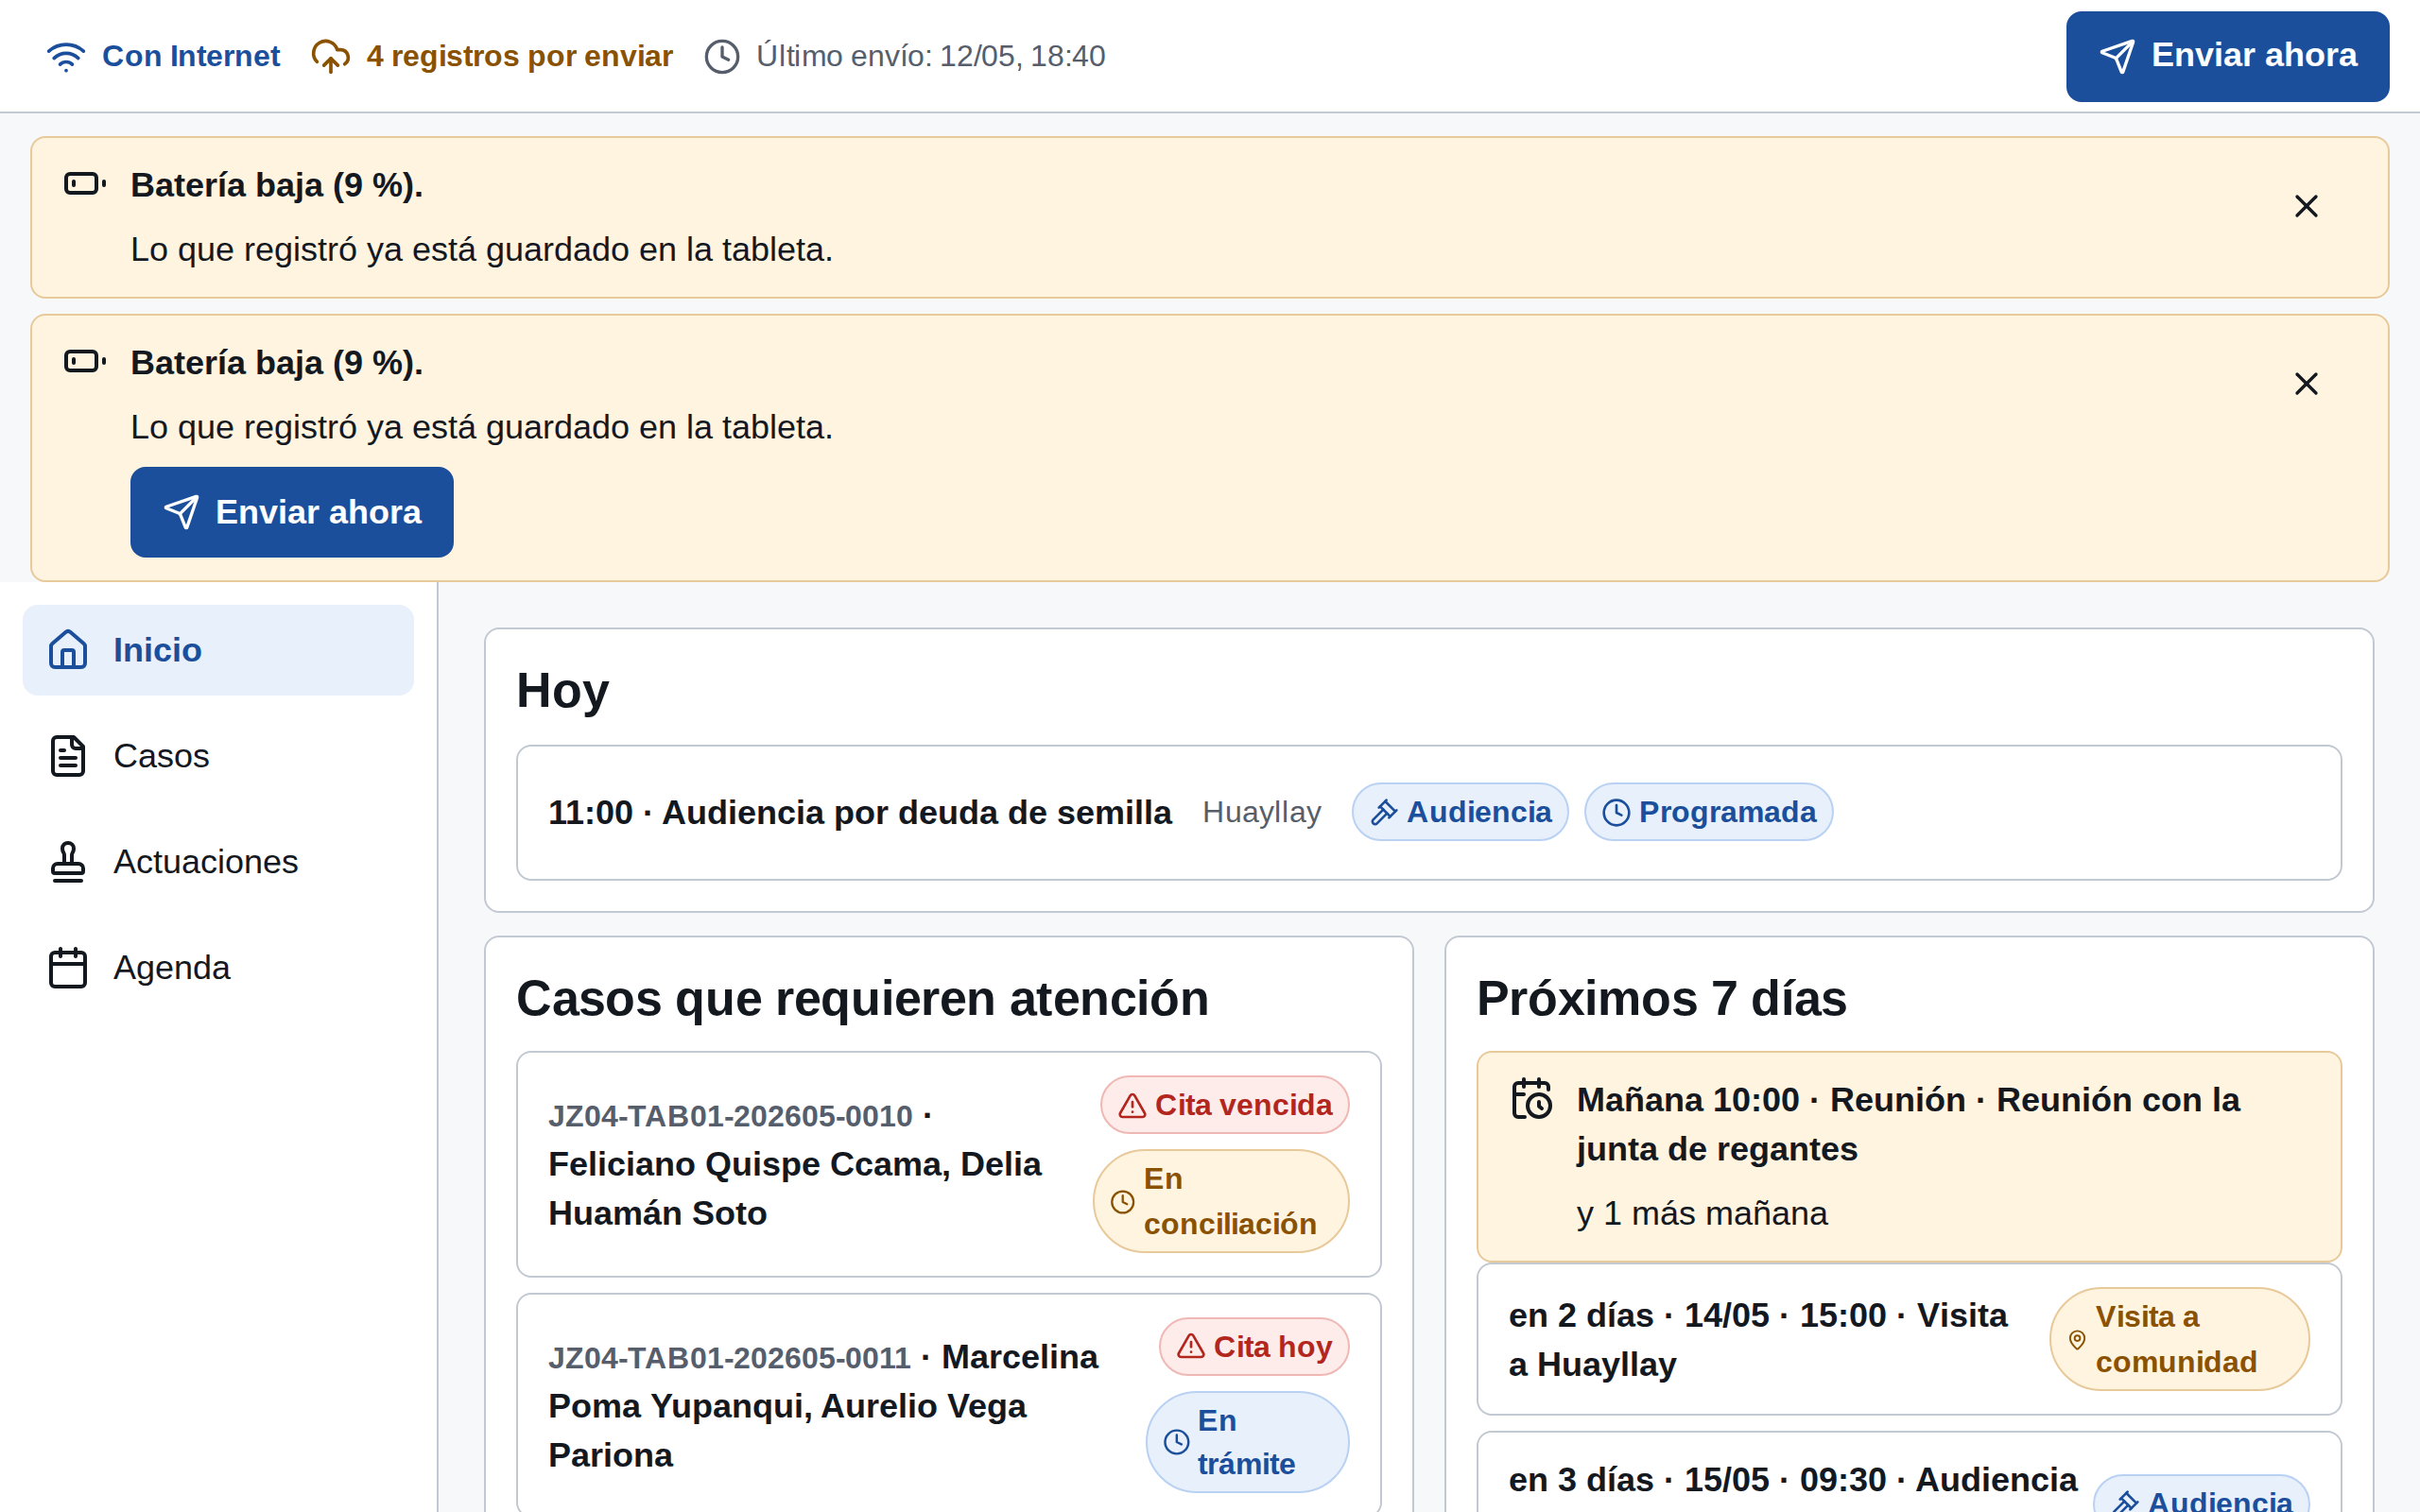
\includegraphics[width=0.78\linewidth]{capturas/X-03_bateria-10.png}
\caption{P-01 · Batería al 10 \%. El mismo aviso, más visible, con la opción de enviar si hay Internet}
\end{figure}
\begin{figure}[H]\centering
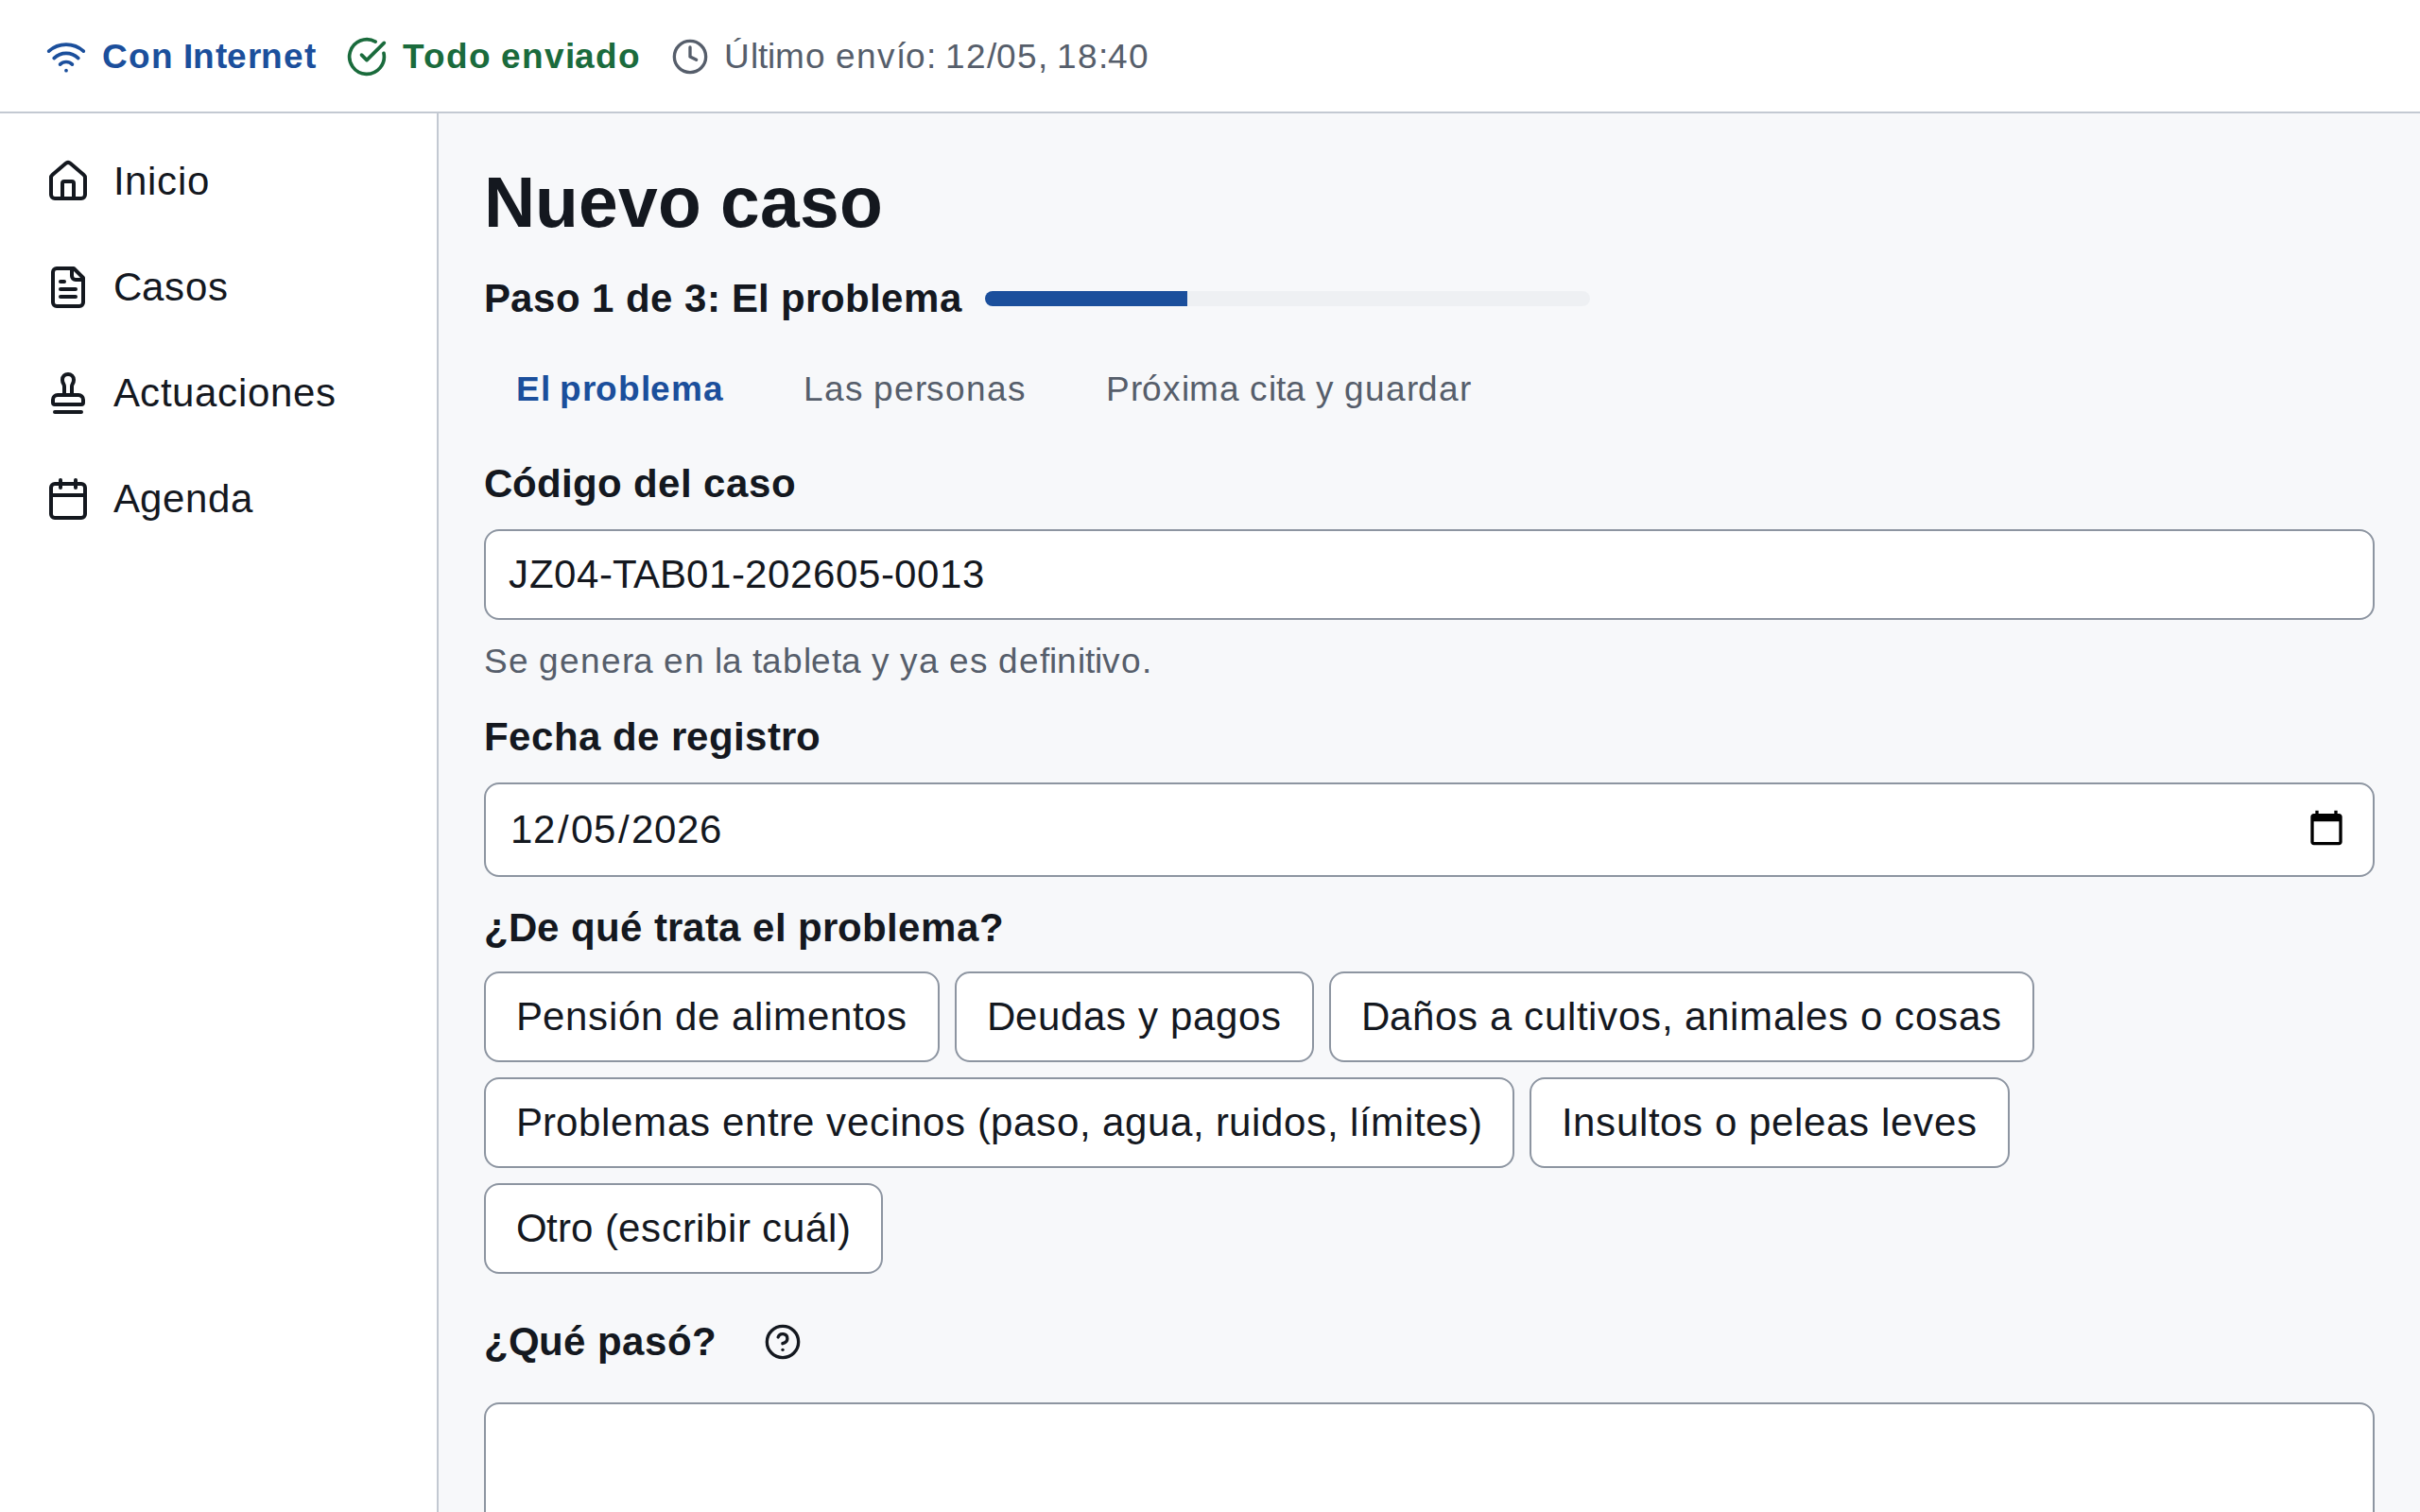
\includegraphics[width=0.78\linewidth]{capturas/X-04_letra-grande.png}
\caption{P-03 · Letra grande. El formulario no se rompe con la letra grande}
\end{figure}
\begin{figure}[H]\centering
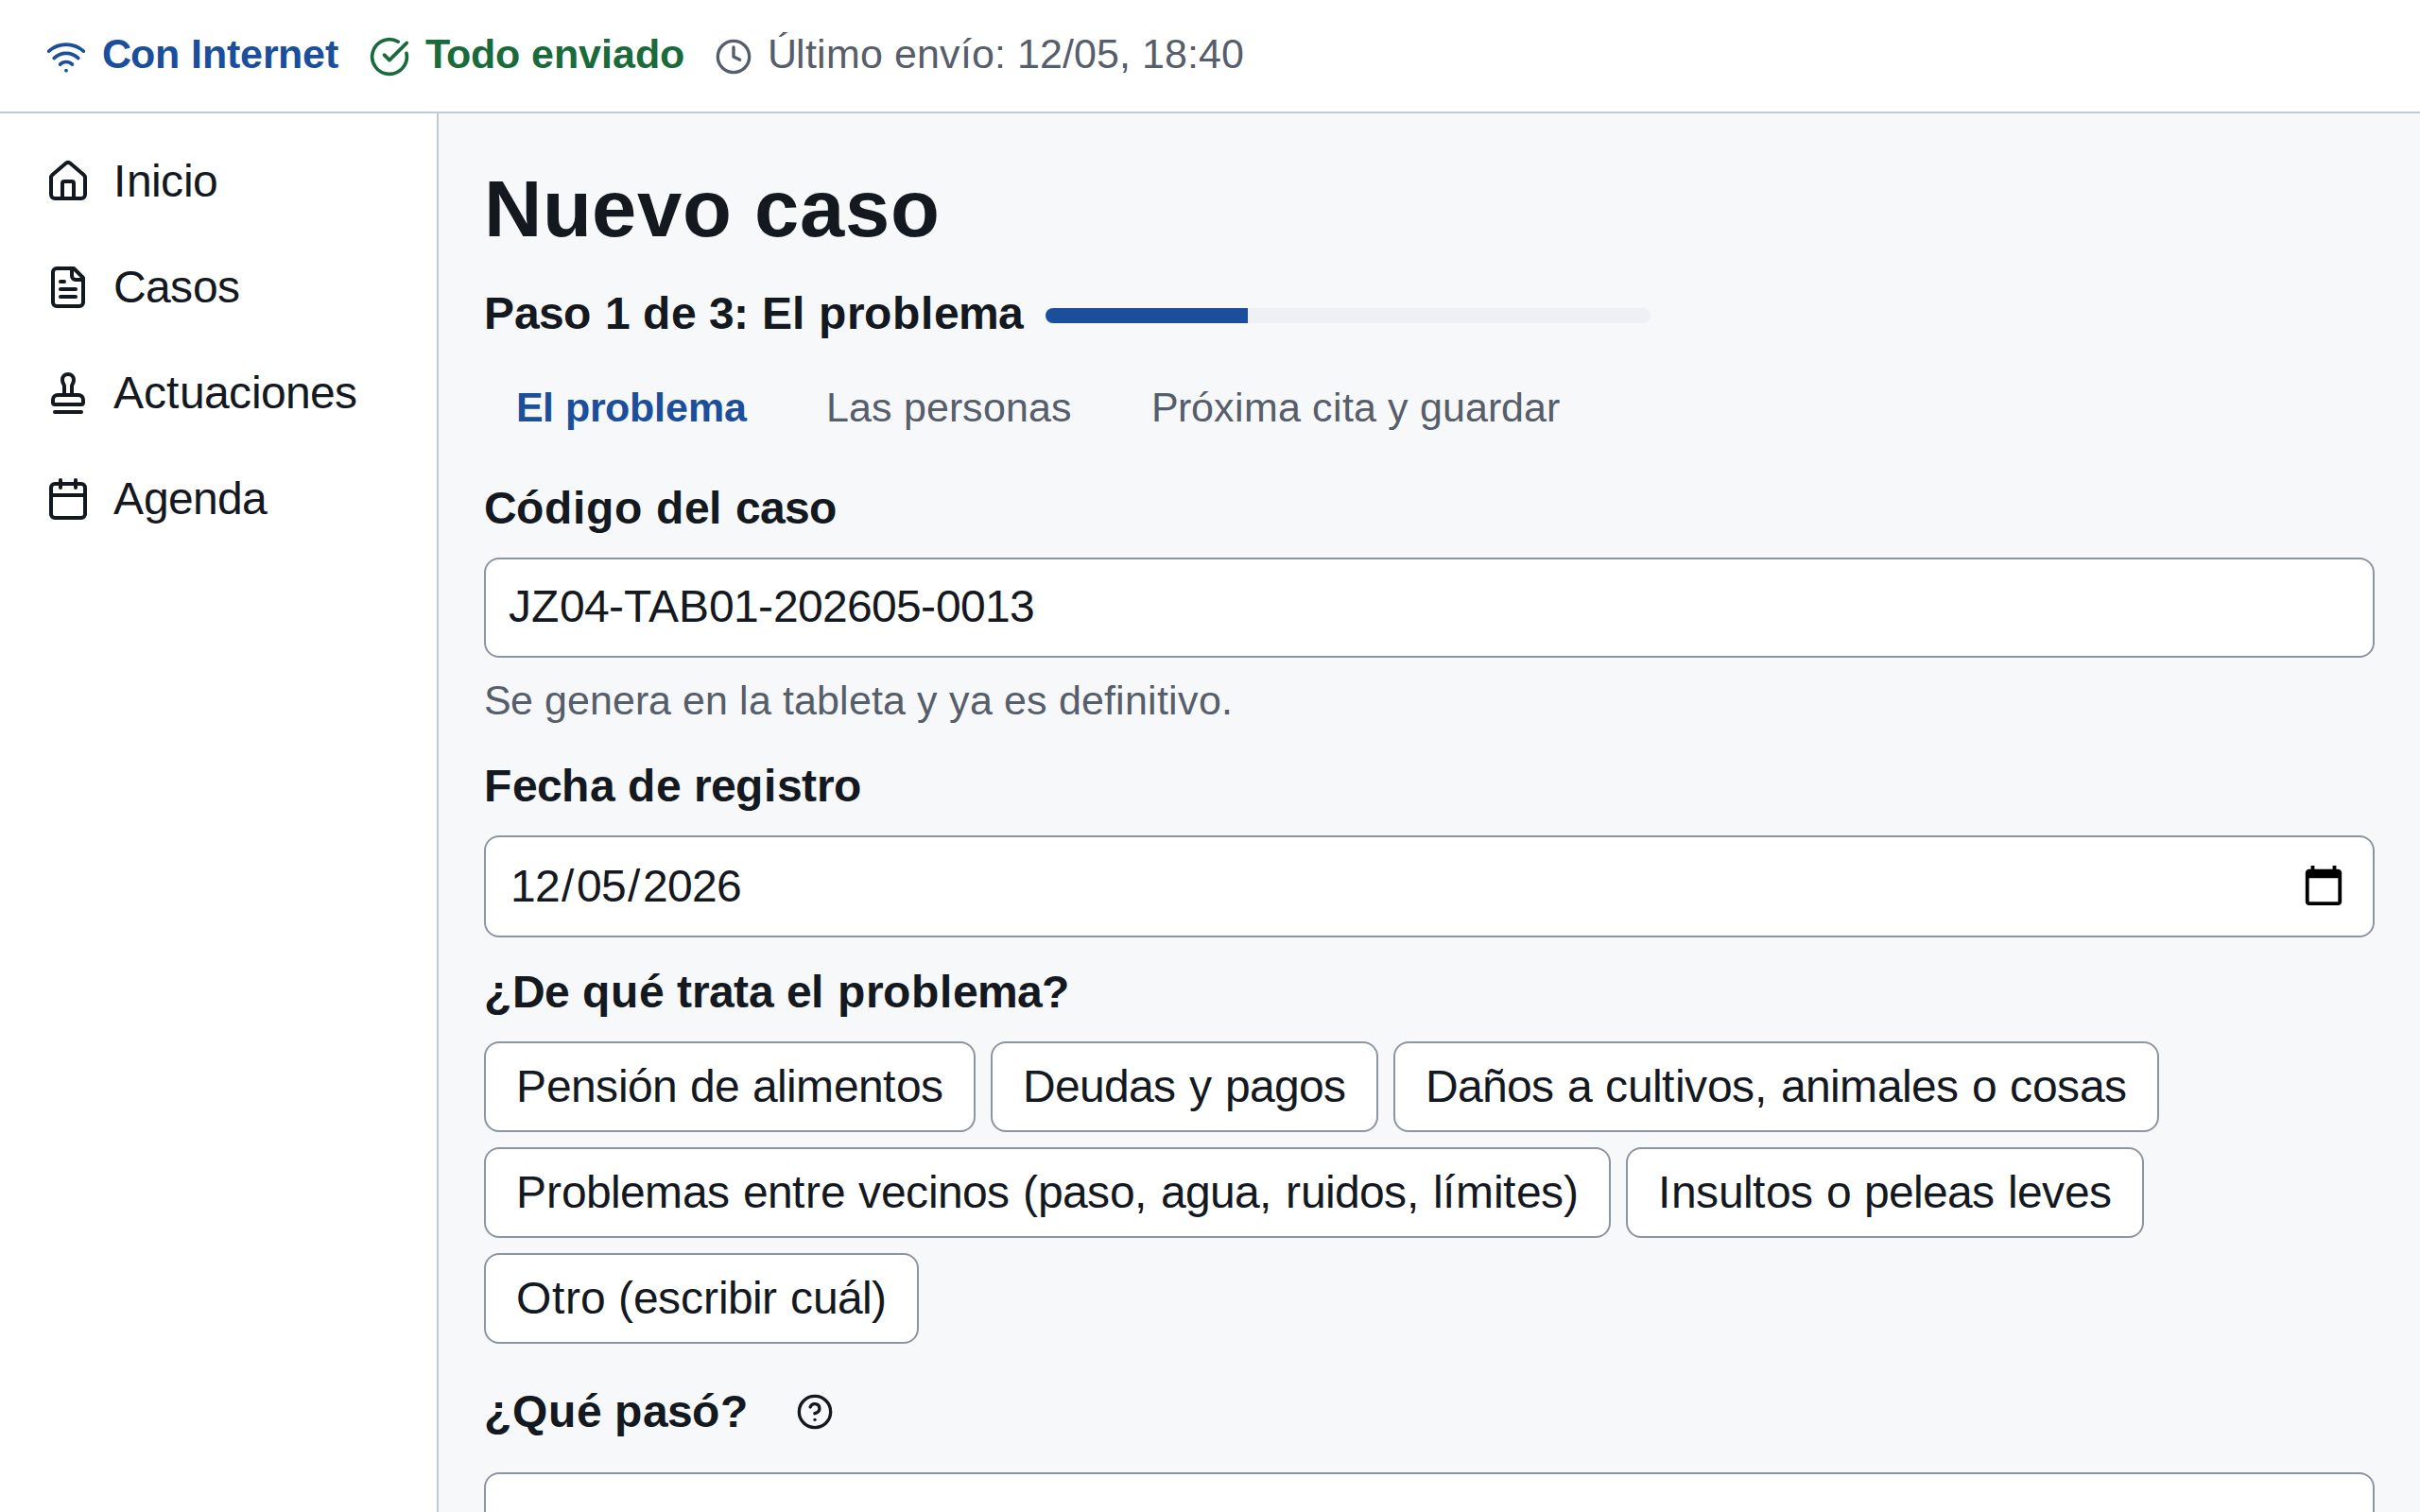
\includegraphics[width=0.78\linewidth]{capturas/X-05_letra-muy-grande.png}
\caption{P-03 · Letra muy grande. Sigue usándose con la letra muy grande, para presbicia}
\end{figure}
\begin{figure}[H]\centering
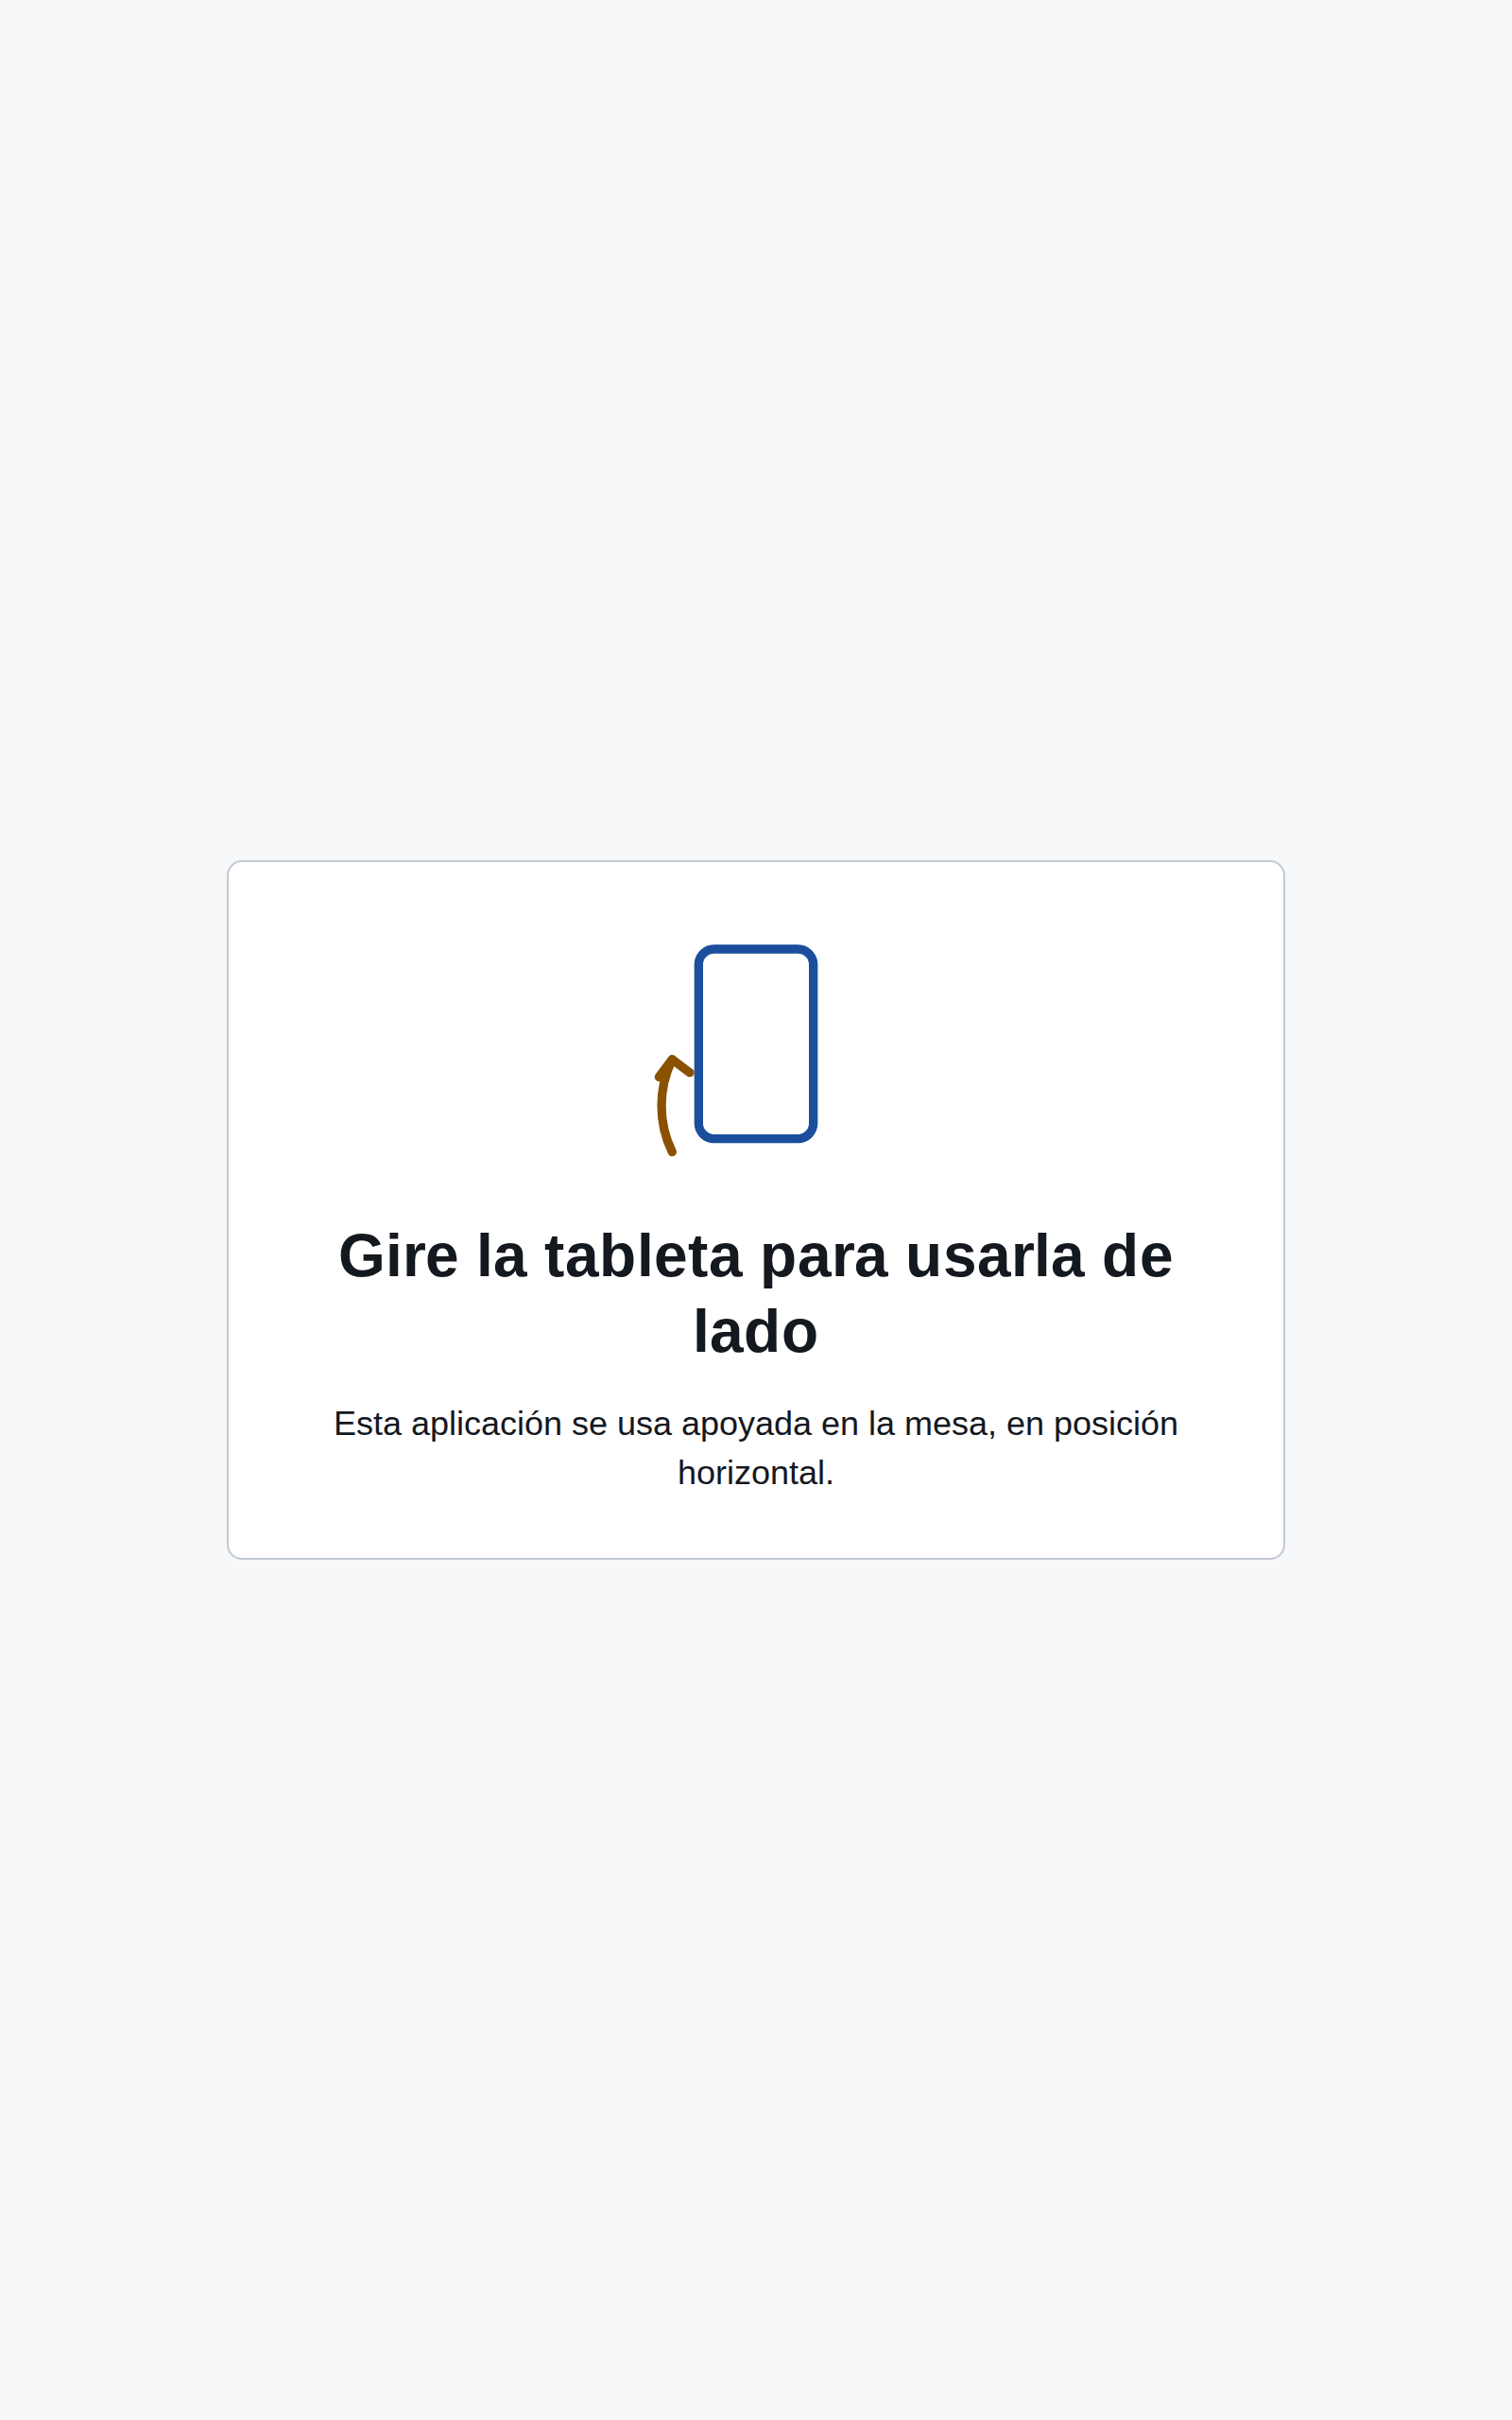
\includegraphics[width=0.78\linewidth]{capturas/X-06_orientacion.png}
\caption{Orientación · Tableta en vertical. Mensaje para girar la tableta, con ilustración, en vez de un diseño roto}
\end{figure}
